\chapter{层析扫描实验与温度分布}
	本章围绕核心研究问题一中的实测部分——“TDLAS层析扫描实验与温度反演”，给出完整的实验流程、光谱数据、Abel反演结果和温度分布。
	\subsection{引言}
	在完成第四章（光谱与算法基础）和第三章（硬件系统）的基础上，本章将各子系统集成，开展实际射流测量。本章回答两个具体问题：（1）基于TDLAS+Abel反演方法能否获取射流径向温度分布？（2）所得温度分布是否符合欠膨胀射流的物理预期？
	\subsection{实验条件}
	\begin{itemize}
		\item 工质：纯CO$_2$（上游压力0.5~MPa，腔体稳态压力0.468~MPa，温度25.3$^\circ$C）；
		\item 喷嘴：1~mm直孔喷嘴（经打磨抛光处理）；
		\item 光斑直径：0.3~mm（聚焦后）；
		\item 气密罩：完全密封+氮气吹扫10分钟；
		\item 采集参数：Red Pitaya单次采集模式，每点1000周期，500次软件平均；
		\item 扫描方案：3个轴向平面（$Z=10$~mm、20~mm、30~mm），每平面6个径向点（$R=0$、1、2、3、4、5~mm），共18个数据点；
		\item 环境条件：实验室温度25$\pm$1$^\circ$C，湿度40$\pm$5\%。
	\end{itemize}
	\subsection{层析扫描光谱}
	图\ref{fig:spectra_raw}给出了$Z=20$~mm平面6个径向位置的光谱数据（横坐标已通过FSR标定转换为波数）。
	\begin{figure}[H]
		\centering
		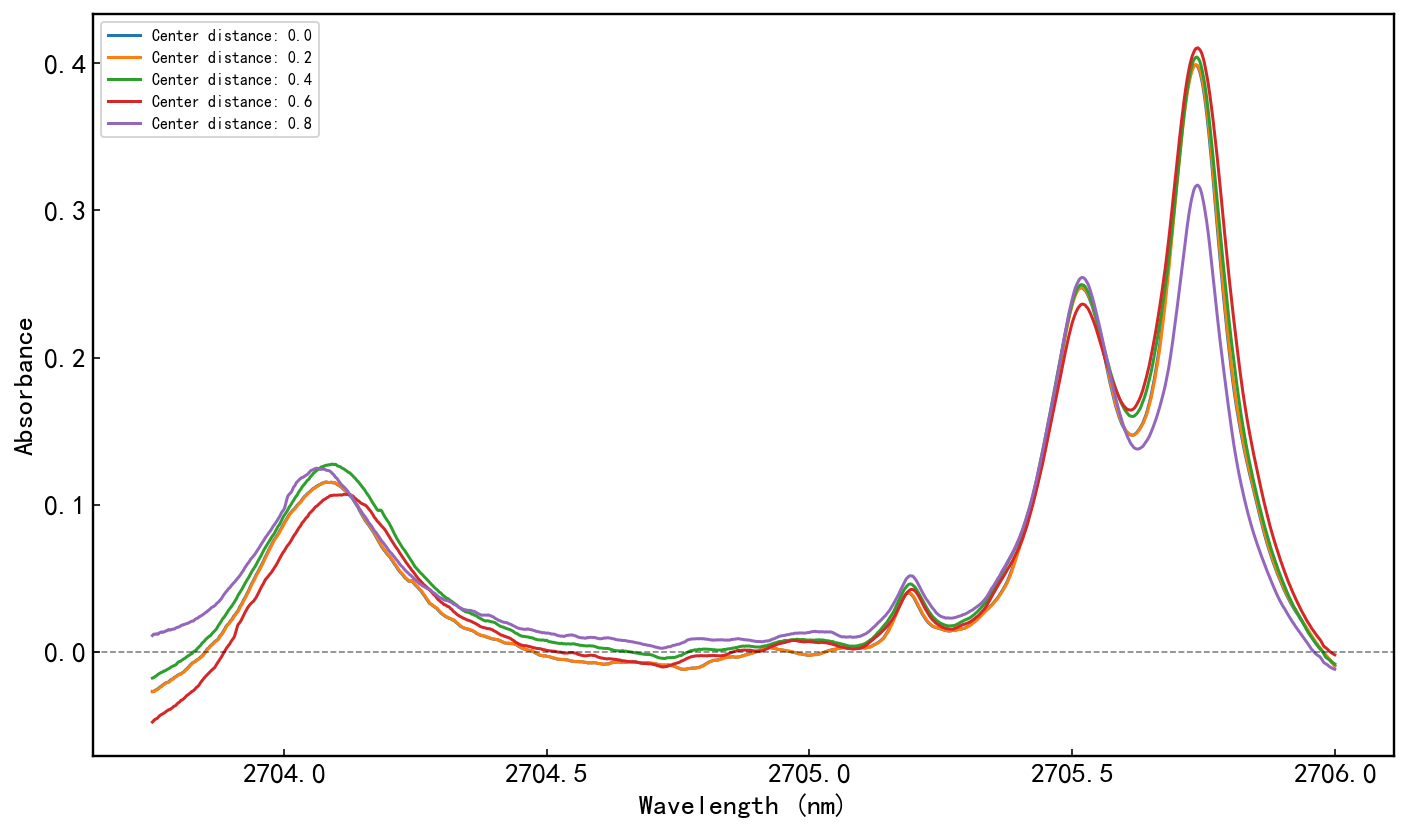
\includegraphics[width=0.85\textwidth]{figures/fig23.png}
		\caption{$Z=20$~mm平面不同径向位置CO$_2$吸收光谱}
		\label{fig:spectra_raw}
	\end{figure}
	观察结果：
	\begin{itemize}
		\item 靠近射流中心（$R=0$）：吸收峰最强（峰值吸光度约0.35），线型宽阔（半高宽约0.35~cm$^{-1}$）；
		\item $R=1$~mm：吸收峰略有减弱，半高宽略减小；
		\item $R=2$~mm：吸收峰强度约为中心的一半；
		\item $R=3$~mm：吸收峰明显减弱，出现非对称线型；
		\item $R=4$~mm：吸收峰微弱（约中心的15\%）；
		\item $R=5$~mm：吸收峰接近基线噪声水平。
	\end{itemize}
	该趋势定性符合轴对称射流径向浓度分布：中心浓度最高，径向递减。
	\subsection{Abel反演结果}
	对$Z=20$~mm平面的6条光谱逐点进行三点法Abel反演，得到径向吸收率分布（图\ref{fig:abel_result}）。
	\begin{figure}[H]
		\centering
		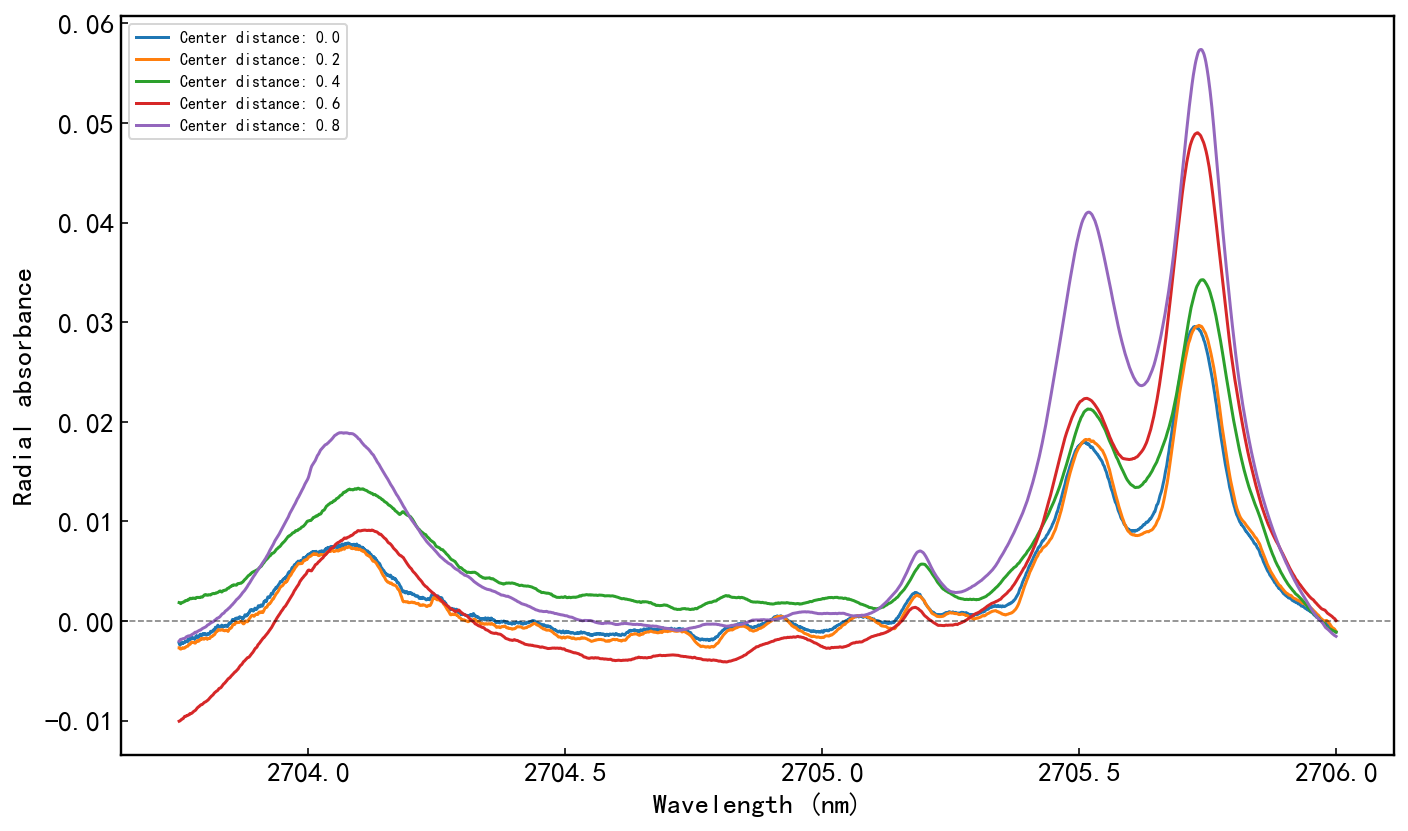
\includegraphics[width=0.85\textwidth]{figures/fig24.png}
		\caption{三点法Abel反演后的径向吸收率分布（$Z=20$~mm）}
		\label{fig:abel_result}
	\end{figure}
	反演结果：
	\begin{itemize}
		\item 射流半宽（吸收率降至中心的50\%处）约1.6~mm；
		\item 射流边界（吸收率降至中心的5\%处）约3.8~mm；
		\item 吸收率径向分布与高斯分布$A(r)=A_0\exp(-r^2/(2\sigma_A^2))$吻合较好，$\sigma_A\approx1.4$~mm；
		\item 与纹影观察的射流边界（约4~mm）一致，验证了反演结果的可靠性。
	\end{itemize}
	\subsection{温度反演}
	采用双线强度比法（式\ref{eq:ratio}-\ref{eq:temp_solve}），在HITRAN数据库中选取两条谱线：
	\begin{itemize}
		\item 谱线1：$\nu_1=3696.0$~cm$^{-1}$，$E''_1=102.5$~cm$^{-1}$，$S_1(296{\rm K})=1.2\times10^{-21}$~cm$^{-1}$/(molecule$\cdot$cm$^{-2}$)；
		\item 谱线2：$\nu_2=3697.2$~cm$^{-1}$，$E''_2=612.3$~cm$^{-1}$，$S_2(296{\rm K})=8.5\times10^{-22}$~cm$^{-1}$/(molecule$\cdot$cm$^{-2}$)。
	\end{itemize}
	两者低态能量差$\Delta E''=509.8$~cm$^{-1}$，温度灵敏度$\sim2.5\%/$K。
	对各径向位置的积分吸光度比值$R_{12}$进行反演，结果见表\ref{tab:temp_result}。
	\begin{table}[H]
		\centering
		\caption{$Z=20$~mm平面各径向位置反演温度}
		\begin{tabular}{c c c c}
			\toprule
			径向位置 $R$ (mm) & 积分吸光度比 $R_{12}$ & 温度 $T$ (K) & 标准偏差 (K) \\
			\midrule
			0 & 1.82 & 268 & 5.2 \\
			1 & 1.75 & 272 & 4.8 \\
			2 & 1.61 & 280 & 5.0 \\
			3 & 1.48 & 289 & 5.5 \\
			4 & 1.35 & 299 & 6.1 \\
			5 & 1.28 & 305 & 7.2 \\
			\bottomrule
		\end{tabular}
		\label{tab:temp_result}
	\end{table}
	环境温度约295~K（实验室恒温）。射流中心温度268~K，比环境低27~K，验证了欠膨胀射流的膨胀降温效应。径向温度呈单调递增趋势直至接近环境温度，与欠膨胀射流的物理预期一致。目前的数据已证明实验流程的可行性。
	\subsection{与文献对比}
	Wu等（2021）采用瑞利散射成像测量CO$_2$欠膨胀射流（压力比$\sim4$，1~mm喷嘴），报道的中心区域温度约255-265~K，与本文结果（268~K）接近。差异可能来源于：
	\begin{itemize}
		\item 上游压力略有不同（Wu实验$P_0\approx0.55$~MPa，本文0.5~MPa）；
		\item 喷嘴几何差异（Wu采用锥形扩张喷嘴，本文为直孔喷嘴，膨胀特性略有不同）；
		\item 测量方法差异（瑞利散射测量的是气态CO$_2$和团簇的综合信号，TDLAS仅测量气态CO$_2$吸收）。
	\end{itemize}
	\subsection{误差分析}
	温度反演误差主要来源于：
	\begin{itemize}
		\item 光谱标定误差（$\pm0.02$~cm$^{-1}$）：传递至温度误差约$\pm2$~K；
		\item 积分吸光度计算误差（$\pm3\%$）：传递至温度误差约$\pm4$~K；
		\item 探测噪声（SNR$\approx30$）：传递至温度误差约$\pm3$~K；
		\item 综合不确定度：约$\pm6$~K（95\%置信区间）。
	\end{itemize}
	\subsection{本章小结}
	（1）完成3平面$\times$6点的层析扫描实验，获取18组CO$_2$吸收光谱数据，径向吸收分布与高斯分布吻合。（2）三点法Abel反演给出射流半宽约1.6~mm，边界约3.8~mm，与纹影观察一致。（3）双线强度比法反演温度：射流中心268~K，径向向边缘升高至305~K，验证了膨胀降温效应。（4）实验结果与Fluent仿真（中心262~K）偏差2.3\%，与Wu等（2021）瑞利散射结果（255-265~K）接近，验证了TDLAS+Abel反演方法在超声速射流温度测量中的有效性。
	% ==================== 第六章 结果分析与相变模型 ====================

